\chapter[Solução Desenvolvida: Automatização do Processo de Inscrição no MOA]{Solução Desenvolvida: Automatização do Processo de Inscrição no MOA}
\label{chap:solucao}
	Uma vez que a modelagem do TO-BE foi realizada, verificou-se a necessidade de adaptá-lo a um nível de abstração mais distante do negócio e mais próximo de uma aplicação a ser desenvolvida. Dessa forma, mantendo a coerência em relação às atividades e suas sequências, foi elaborado um modelo voltado para a solução, onde através dele seria possível levantar a aplicação em um servidor contendo a automação do processo desenvolvido. Esse modelo conta com algumas diferenças em relação ao modelo TO-BE de negócio, entre elas a inclusão de eventos intermediários onde o status da solicitação é alterado conforme comportamento nas atividades.
	\begin{figure}[H]
		\centering
		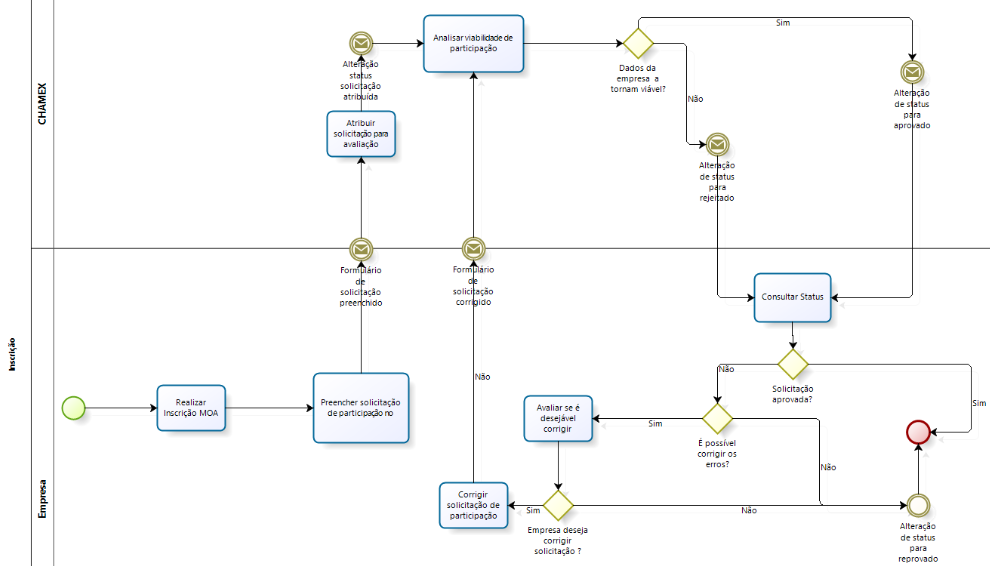
\includegraphics[scale=0.6]{solucao_01}
		\caption[Solução do Processo de Inscrição no MOA]{Solução do Processo de Inscrição no MOA.}
		\label{fig:solprocesso}
	\end{figure}
	Também pode ser observado na Figura \ref{fig:solprocesso} a inclusão da atividade \textbf{Corrigir Solicitação de Participação}, diferentemente do modelo de negócio onde o preenchimento de uma solicitação, sendo de correção ou não, pertencia à mesma atividade. Como já citado anteriormente, esse modelo possibilitou grande avanço em relação ao preenchimento e aferição dos questionários, trazendo para regras que antigamente eram validadas de forma manual, como pode ser visto nos resultados da execução do modelo desenvolvido.
	\begin{figure}[H]
		\centering
		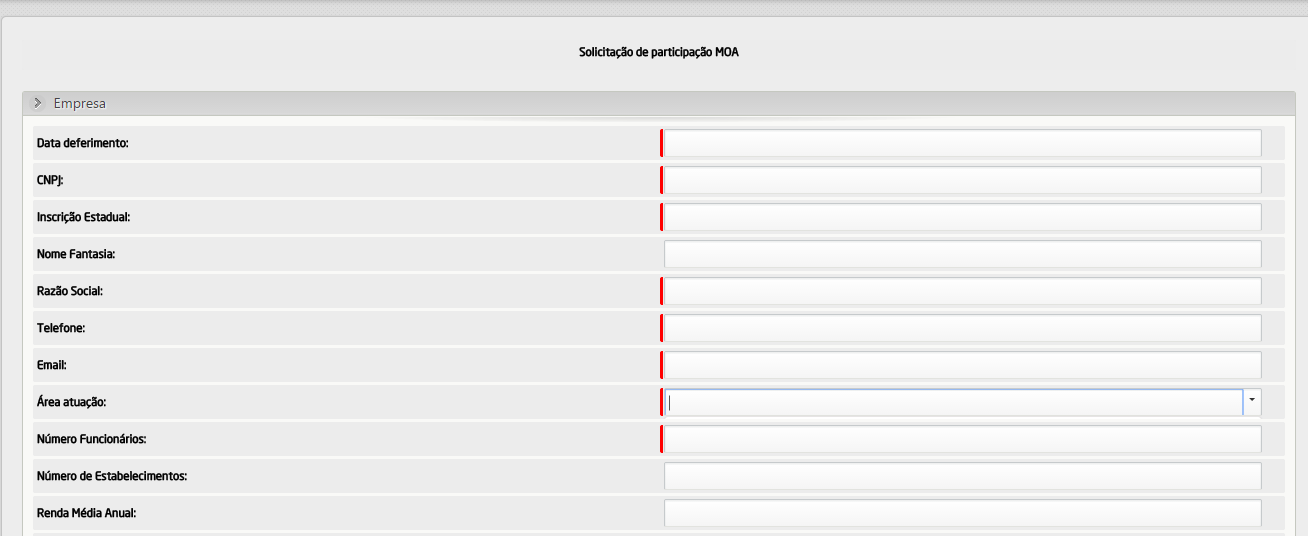
\includegraphics[scale=0.46]{solucao_02}
		\caption[Preenchimento da Solicitação de Inscrição no MOA, Solução Desenvolvida]{Preenchimento da Solicitação de Inscrição no MOA, Solução Desenvolvida.}
		\label{fig:solinscricaoimagem}
	\end{figure}
	\begin{figure}[H]
		\centering
		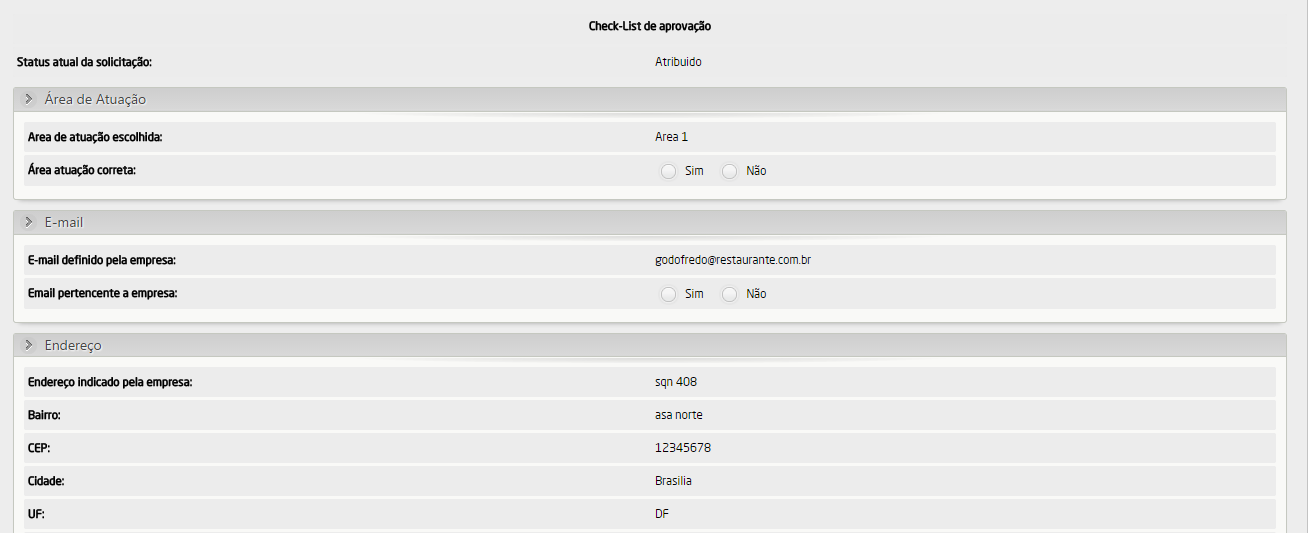
\includegraphics[scale=0.46]{solucao_03}
		\caption[Preenchimento do \emph{Check-list} do Analista, Solução Desenvolvida]{Preenchimento do \emph{Check-list} do Analista, Solução Desenvolvida.}
		\label{fig:solchecklistimagem}
	\end{figure}
	Regras de negócios capazes de alterar a sequência das atividades também foram automatizadas, como por exemplo, o fato da empresa não ter sua solicitação aprovada caso esteja em débito com a receita, ou no descumprimento de qualquer dado apresentado na Figura \ref{fig:regranegocio}.
	\begin{figure}[H]
		\centering
		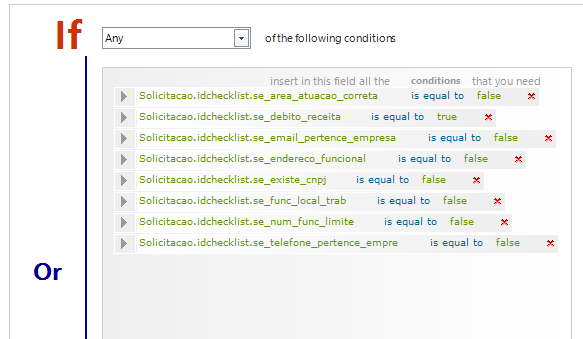
\includegraphics[scale=1]{regra_negocio}
		\caption[Regras de Negócio para Análise da Solicitação]{Regras de Negócio para Análise da Solicitação.}
		\label{fig:regranegocio}
	\end{figure}
	Outro elemento importante criado na automação foi a capacidade de alterar status da solicitação, conforme o contexto indica. Seguindo os passos da figura anterior e assumindo que a solicitação da empresa tenha descumprido uma dessas regras, o status da sua solicitação é alterado para rejeitado, dando a ela possibilidade de correção dos dados. Essa alteração no status pode ser verificada na Figura \ref{fig:mudancastatus}.
	\begin{figure}[H]
		\centering
		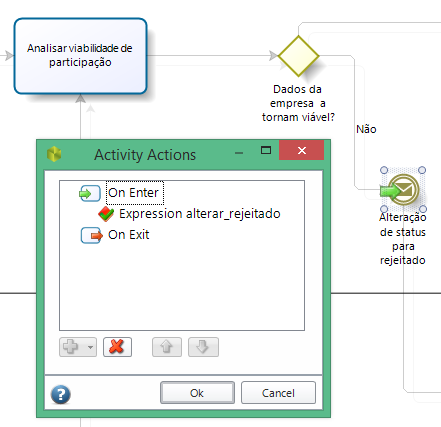
\includegraphics[scale=1]{mudanca_status}
		\caption[Alteração para \emph{Status} Rejeitado]{Alteração para \emph{Status} Rejeitado.}
		\label{fig:mudancastatus}
	\end{figure}
	É importante definir a qual papel está associada cada atividade. Dentro do contexto que envolve o processo de inscrição no MOA foram identificados três papeis:
	\begin{itemize}
		\item{\textbf{Gerente da CHAMEX}: Resposável por atribuir uma solicitação à um determinado analista;}
		\item{\textbf{Analista de Solicitações do MOA}: Responsável por analisar a solicitação enviada pela empresa solicitante e preencher um \emph{check-list} de acordo com as informações do formulário de solicitação.}
		\item{\textbf{Empresa Solicitante}: Empresa que deseja solicitar participação no MOA.}
	\end{itemize}
	\ \indent A Figura \ref{fig:atribuicaopapel} retrata a atribuição de papéis para as atividades no contexto da automação da solução na ferramenta BPMS.
	\begin{figure}[H]
		\centering
		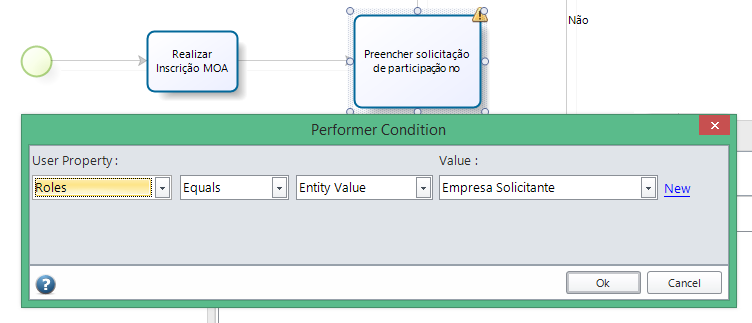
\includegraphics[scale=0.8]{atribuicao_papel}
		\caption[Atribuições de Papéis para Atividades, Solução BPMS]{Atribuições de Papéis para Atividades, Solução BPMS.}
		\label{fig:atribuicaopapel}
	\end{figure}
	Cada atividade vinculada a um papel só pode ser realizada por ele. Dessa forma, foram criados usuários fictícios na aplicação pertencentes a um papel. Dessa forma, a segurança sobre quem realizava cada trabalho estava garantida.
	\\ \indent Para suportar os dados preenchidos nos formulários e garantir sua integridade em relação aos seus relacionamentos, foi modelado um banco de dados que pudesse refletir os dados e os relacionamentos da aplicação. O banco de dados modelado é apresentado na Figura \ref{fig:bdbpms}.
	\begin{figure}[H]
		\centering
		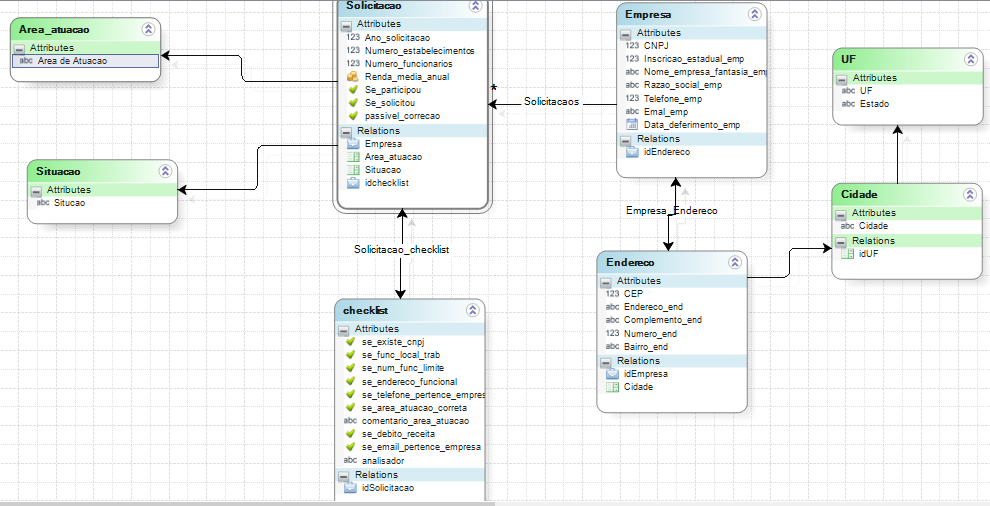
\includegraphics[scale=0.58]{modelagem_banco}
		\caption[Modelo de Entidade-Relacionamento de Banco de Dados Desenvolvido]{Modelo de Entidade-Relacionamento de Banco de Dados Desenvolvido.}
		\label{fig:bdbpms}
	\end{figure}
	Como definido como objetivo na identificação de pontos de automação, é possível criar validações em tempo real no formulário, diferentemente do que ocorria anteriormente com o uso do aplicativo Excel. Um campo em branco, por exemplo, ou um campo numérico sendo preenchido com letras não pode ocorrer mais. Como dito, essa melhoria por si só já antecede para o preenchimento do formulário trabalhos que eram realizados anteriormente de forma mais complexa e manual em atividades posteriores, em validações manuais feitas por um analista. Dessa forma, o \emph{check-list} tornou-se menor e mais focado em ações de validações que não podem ser feitas de maneira automática.
	\\ \indent Mais detalhes a respeito da automação são tratados na \textbf{Seção \ref{sec:planejamento_desenvolvimento} - \nameref{sec:planejamento_desenvolvimento}}, onde é realizado um mapeamento entre histórias de usuários elicitadas e tarefas desenvolvidas.